
\section{Fibonacci $S$-matrix}
Recall the Fibonacci theory which we introduced in sections 8.2.1 and 10.2.1.
\begin{enumerate}
\item First let us pretend that we have not calculated the $R$-matrices or $\theta _{\tau }$, i.e., we do not know the braiding phases or the twist factors. We only know the fusion rules $\tau \times \tau =I+\tau $. Using the quantum dimensions, we can obtain three out of four elements of the 2 by $2S$-matrix. Determine the remaining elment of the $S$-matrix by enforcing unitarity.
\item Given the twist factor $\theta _{\tau } =\mathrm{e}^{\pm 4\pi \mathrm{i} /5}$ (With $\pm $ being for right or lefthanded theories), calculate the $S$-matrix explicitly by using Eq. 17.20.
\end{enumerate}

\paragraph{Answer}

\section{Using the pivotal property}
Use the pivotal property (Section 14.8.1) to demonstrate the identity shown in Fig. \ref{fig:PivotalPropertyIdentity}. 
\begin{figure}[h!]
\centering
\tikzset{every picture/.style={line width=0.75pt}} %set default line width to 0.75pt        

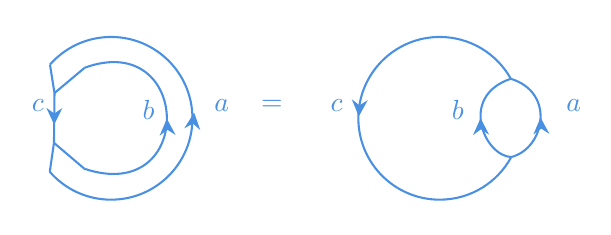
\begin{tikzpicture}[x=0.75pt,y=0.75pt,yscale=-1,xscale=1]
%uncomment if require: \path (0,86); %set diagram left start at 0, and has height of 86

%Shape: Arc [id:dp22047988155782305] 
\draw  [draw opacity=0] (211.79,16.39) .. controls (218.97,8.22) and (229.5,3.07) .. (241.23,3.07) .. controls (262.88,3.07) and (280.43,20.62) .. (280.43,42.27) .. controls (280.43,63.92) and (262.88,81.47) .. (241.23,81.47) .. controls (229.45,81.47) and (218.88,76.27) .. (211.69,68.04) -- (241.23,42.27) -- cycle ; \draw  [color={rgb, 255:red, 74; green, 144; blue, 226 }  ,draw opacity=1 ] (211.79,16.39) .. controls (218.97,8.22) and (229.5,3.07) .. (241.23,3.07) .. controls (262.88,3.07) and (280.43,20.62) .. (280.43,42.27) .. controls (280.43,63.92) and (262.88,81.47) .. (241.23,81.47) .. controls (229.45,81.47) and (218.88,76.27) .. (211.69,68.04) ;  
%Straight Lines [id:da21244688064449924] 
\draw [color={rgb, 255:red, 74; green, 144; blue, 226 }  ,draw opacity=1 ]   (228.53,17.89) -- (213.97,30.1) ;
%Straight Lines [id:da1553454512319279] 
\draw [color={rgb, 255:red, 74; green, 144; blue, 226 }  ,draw opacity=1 ]   (211.79,16.39) -- (213.97,30.1) ;
%Straight Lines [id:da8377047223627767] 
\draw [color={rgb, 255:red, 74; green, 144; blue, 226 }  ,draw opacity=1 ]   (213.72,54.1) -- (228.38,66.57) ;
%Straight Lines [id:da6533569501785481] 
\draw [color={rgb, 255:red, 74; green, 144; blue, 226 }  ,draw opacity=1 ]   (213.72,54.1) -- (211.69,68.04) ;
%Straight Lines [id:da6644484377436084] 
\draw [color={rgb, 255:red, 74; green, 144; blue, 226 }  ,draw opacity=1 ]   (213.97,30.1) -- (213.72,54.1) ;
\draw [shift={(213.81,45.3)}, rotate = 270.6] [fill={rgb, 255:red, 74; green, 144; blue, 226 }  ,fill opacity=1 ][line width=0.08]  [draw opacity=0] (8.04,-3.86) -- (0,0) -- (8.04,3.86) -- (5.34,0) -- cycle    ;
%Curve Lines [id:da1570096869940174] 
\draw [color={rgb, 255:red, 74; green, 144; blue, 226 }  ,draw opacity=1 ]   (228.53,17.89) .. controls (280.33,-0.9) and (282.33,84.6) .. (228.38,66.57) ;
\draw [shift={(268.11,42.45)}, rotate = 87.4] [fill={rgb, 255:red, 74; green, 144; blue, 226 }  ,fill opacity=1 ][line width=0.08]  [draw opacity=0] (8.04,-3.86) -- (0,0) -- (8.04,3.86) -- (5.34,0) -- cycle    ;
%Straight Lines [id:da3195319441361355] 
\draw [color={rgb, 255:red, 74; green, 144; blue, 226 }  ,draw opacity=1 ]   (280.77,43.94) -- (281.05,41.44) ;
\draw [shift={(281.26,39.51)}, rotate = 96.38] [fill={rgb, 255:red, 74; green, 144; blue, 226 }  ,fill opacity=1 ][line width=0.08]  [draw opacity=0] (8.04,-3.86) -- (0,0) -- (8.04,3.86) -- (5.34,0) -- cycle    ;
%Curve Lines [id:da8394233024581486] 
\draw [color={rgb, 255:red, 74; green, 144; blue, 226 }  ,draw opacity=1 ]   (433.81,23.22) .. controls (455.66,29.94) and (449.99,56.94) .. (433.99,60.94) ;
\draw [shift={(448.16,41.89)}, rotate = 87.28] [fill={rgb, 255:red, 74; green, 144; blue, 226 }  ,fill opacity=1 ][line width=0.08]  [draw opacity=0] (8.04,-3.86) -- (0,0) -- (8.04,3.86) -- (5.34,0) -- cycle    ;
%Curve Lines [id:da25849282059265066] 
\draw [color={rgb, 255:red, 74; green, 144; blue, 226 }  ,draw opacity=1 ]   (433.81,23.22) .. controls (408.66,31.61) and (420.99,60.28) .. (433.99,60.94) ;
\draw [shift={(419.26,42.21)}, rotate = 88.33] [fill={rgb, 255:red, 74; green, 144; blue, 226 }  ,fill opacity=1 ][line width=0.08]  [draw opacity=0] (8.04,-3.86) -- (0,0) -- (8.04,3.86) -- (5.34,0) -- cycle    ;
%Shape: Arc [id:dp5891124208443936] 
\draw  [draw opacity=0] (433.99,61.03) .. controls (427.34,73.21) and (414.42,81.47) .. (399.57,81.47) .. controls (377.92,81.47) and (360.37,63.92) .. (360.37,42.27) .. controls (360.37,20.62) and (377.92,3.07) .. (399.57,3.07) .. controls (414.21,3.07) and (426.98,11.1) .. (433.71,23) -- (399.57,42.27) -- cycle ; \draw  [color={rgb, 255:red, 74; green, 144; blue, 226 }  ,draw opacity=1 ] (433.99,61.03) .. controls (427.34,73.21) and (414.42,81.47) .. (399.57,81.47) .. controls (377.92,81.47) and (360.37,63.92) .. (360.37,42.27) .. controls (360.37,20.62) and (377.92,3.07) .. (399.57,3.07) .. controls (414.21,3.07) and (426.98,11.1) .. (433.71,23) ;  
%Straight Lines [id:da893350250219167] 
\draw [color={rgb, 255:red, 74; green, 144; blue, 226 }  ,draw opacity=1 ]   (360.83,37.18) -- (360.72,39.1) ;
\draw [shift={(360.59,41.34)}, rotate = 273.3] [fill={rgb, 255:red, 74; green, 144; blue, 226 }  ,fill opacity=1 ][line width=0.08]  [draw opacity=0] (8.04,-3.86) -- (0,0) -- (8.04,3.86) -- (5.34,0) -- cycle    ;

% Text Node
\draw (201.55,31.86) node [anchor=north west][inner sep=0.75pt]  [color={rgb, 255:red, 74; green, 144; blue, 226 }  ,opacity=1 ]  {$c$};
% Text Node
\draw (254.96,31.86) node [anchor=north west][inner sep=0.75pt]  [color={rgb, 255:red, 74; green, 144; blue, 226 }  ,opacity=1 ]  {$b$};
% Text Node
\draw (289.46,31.86) node [anchor=north west][inner sep=0.75pt]  [color={rgb, 255:red, 74; green, 144; blue, 226 }  ,opacity=1 ]  {$a$};
% Text Node
\draw (459.13,31.86) node [anchor=north west][inner sep=0.75pt]  [color={rgb, 255:red, 74; green, 144; blue, 226 }  ,opacity=1 ]  {$a$};
% Text Node
\draw (403.96,31.86) node [anchor=north west][inner sep=0.75pt]  [color={rgb, 255:red, 74; green, 144; blue, 226 }  ,opacity=1 ]  {$b$};
% Text Node
\draw (345.55,31.86) node [anchor=north west][inner sep=0.75pt]  [color={rgb, 255:red, 74; green, 144; blue, 226 }  ,opacity=1 ]  {$c$};
% Text Node
\draw (312,31.99) node [anchor=north west][inner sep=0.75pt]  [color={rgb, 255:red, 74; green, 144; blue, 226 }  ,opacity=1 ]  {$=$};
\end{tikzpicture}
\caption{This identity can be shown without full isotopy invariance by using the pivotal property.}
\label{fig:PivotalPropertyIdentity}
\end{figure}

You should not assume full isotopy invariance. Nor should you assume $\epsilon =+1$ for any of the particles.

\paragraph{Answer}

\section{Symmetries of $S$}
Use isotopy of diagrams and Hermitian conjugation of diagrams to show the identities in Eq. 17.7.

\paragraph{Answer}

\section{Evaluation of the $S$-link}

\begin{enumerate}
\item Use the $R$-matrices and Eq. 15.4 to derive the value of the matrix $\tilde{S}_{ax}$ (See Fig. 17.2) in terms of fusion multiplicities, twist factors $\theta _{a}$, and the quantum dimensions $\mathsf{d}_{a}$.
\item From your result show that\begin{equation*}
\tikzset{every picture/.style={line width=0.75pt}} %set default line width to 0.75pt        
\begin{tikzpicture}[x=0.75pt,y=0.75pt,yscale=-1,xscale=1, baseline=(XXXX.south) ]
\path (0,91);\path (160.98513793945312,0);\draw    ($(current bounding box.center)+(0,0.3em)$) node [anchor=south] (XXXX) {};
%Shape: Arc [id:dp43240405597707143] 
\draw  [draw opacity=0] (75.76,16.16) .. controls (83.41,24.01) and (88.13,34.74) .. (88.13,46.56) .. controls (88.13,70.62) and (68.62,90.13) .. (44.56,90.13) .. controls (20.5,90.13) and (1,70.62) .. (1,46.56) .. controls (1,22.5) and (20.5,3) .. (44.56,3) .. controls (54.25,3) and (63.21,6.16) .. (70.44,11.52) -- (44.56,46.56) -- cycle ; \draw  [color={rgb, 255:red, 74; green, 144; blue, 226 }  ,draw opacity=1 ] (75.76,16.16) .. controls (83.41,24.01) and (88.13,34.74) .. (88.13,46.56) .. controls (88.13,70.62) and (68.62,90.13) .. (44.56,90.13) .. controls (20.5,90.13) and (1,70.62) .. (1,46.56) .. controls (1,22.5) and (20.5,3) .. (44.56,3) .. controls (54.25,3) and (63.21,6.16) .. (70.44,11.52) ;  
%Shape: Arc [id:dp4575637955931797] 
\draw  [draw opacity=0] (71.27,75.87) .. controls (63.67,68.03) and (59,57.34) .. (59,45.56) .. controls (59,21.5) and (78.5,2) .. (102.56,2) .. controls (126.62,2) and (146.13,21.5) .. (146.13,45.56) .. controls (146.13,69.62) and (126.62,89.13) .. (102.56,89.13) .. controls (92.94,89.13) and (84.04,86.01) .. (76.83,80.72) -- (102.56,45.56) -- cycle ; \draw  [color={rgb, 255:red, 74; green, 144; blue, 226 }  ,draw opacity=1 ] (71.27,75.87) .. controls (63.67,68.03) and (59,57.34) .. (59,45.56) .. controls (59,21.5) and (78.5,2) .. (102.56,2) .. controls (126.62,2) and (146.13,21.5) .. (146.13,45.56) .. controls (146.13,69.62) and (126.62,89.13) .. (102.56,89.13) .. controls (92.94,89.13) and (84.04,86.01) .. (76.83,80.72) ;  
% Text Node
\draw (91,35.5) node [anchor=north west][inner sep=0.75pt]    {$a$};
% Text Node
\draw (148,36.5) node [anchor=north west][inner sep=0.75pt]    {$b$};
\end{tikzpicture}
=\sum _{c} N_{a\overline{b}}^{c}\frac{\theta _{c}}{\theta _{a} \theta _{b}}\mathsf{d}_{c}
\end{equation*}
\end{enumerate}

Note that this diagram differs from $S_{ab}$ by a factor of $Z(S^{3} )=1/\mathcal{D}$.

\paragraph{Answer}

\section{Theories with one nontrivial particle}
Consider an anyon theory with only the identity and one nontrivial particle type $a$ having twist factor $\theta _{s}$. The only possible fusion rules are $s\times s=I+ms$ for some integer $m$ (the semion model is $m=0$ the Fibonacci model is $m=1$ ). Calculate $\mathrm{d}_{s}$ and $\mathcal{D}$ from the fusion rules. Use Eq. 17.20 to calculate the $S$ matrix in terms of $\theta _{s}$. Show that this matrix cannot be unitary for any $m >1$. This justifies that on table 17.1 there are only two types of theory with one nontrivial particle.

\paragraph{Answer}

\section{Product theories[Easy]}
Given two anyon theories $A$ and $B$ with corresponding $S$-matrices $S_{A}$ and $S_{B}$
\begin{enumerate}
\item Show that the product theory $A\times B$ has $S$-matrix $S_{A} \otimes S_{B}$.
\item Show that $A\times B$ is modular if and only if both $A$ and $B$ are modular.
\item Show that the central charge of the product theory is the sum of the central charges of the constituent theories. I.e.,\begin{equation*}
c_{A\times B} =( c_{A} +c_{B})\bmod 8
\end{equation*}
\end{enumerate}

In fact, central charges strictly add in product theories. However, we have only defined the central charge mod 8 so far!

\paragraph{Answer}

\section{Probability of Fusion Channels}
Consider a modular anyon theory on a sphere with a very large number of quasiparticles of all types.
\begin{enumerate}
\item Divide these anyons randomly into two large groups. Show that the probability that the two groups have overall fusion channels $a$ and $\overline{a}$ is given by\begin{equation*}
p(a,\bar{a} )=\mathsf{d}_{a}^{2} /\mathcal{D}^{2}
\end{equation*}Hint: You are counting the total number of fusion trees. Use the strategy of section 8.3 along with the Verlinde formula, and the knowledge that $S_{0b} /S_{00} \geq $ $| S_{xb} /S_{xb}| $ for all $x$. (You may start by assuming this is strictly $ >$ and worry about the $\geq $ case later).
\item Instead divide the anyons randomly into three large groups. Show that the probability that the groups have overall fusion channels $a,b,c$ is given by\begin{equation*}
p(a,b,c)=N_{abc}\mathsf{d}_{a}\mathsf{d}_{b}\mathsf{d}_{c} /\mathcal{D}^{4}
\end{equation*}
\item Finally try four large groups. Show that the probability that the groups have overall fusion channels $a,b,c,f$ is given by\begin{equation*}
p(a,b,c,f)=N_{abcf}\mathsf{d}_{a}\mathsf{d}_{b}\mathsf{d}_{c}\mathsf{d}_{f} /\mathcal{D}^{6}
\end{equation*}where $N_{abcf}$ is the number of ways $a,b,c$ and $f$ can fuse to the vacuum.
\end{enumerate}

\paragraph{Answer}



